\chapter{Anhang}

\begin{figure}
	\centering
	\begin{subfigure}{0.48\textwidth}
		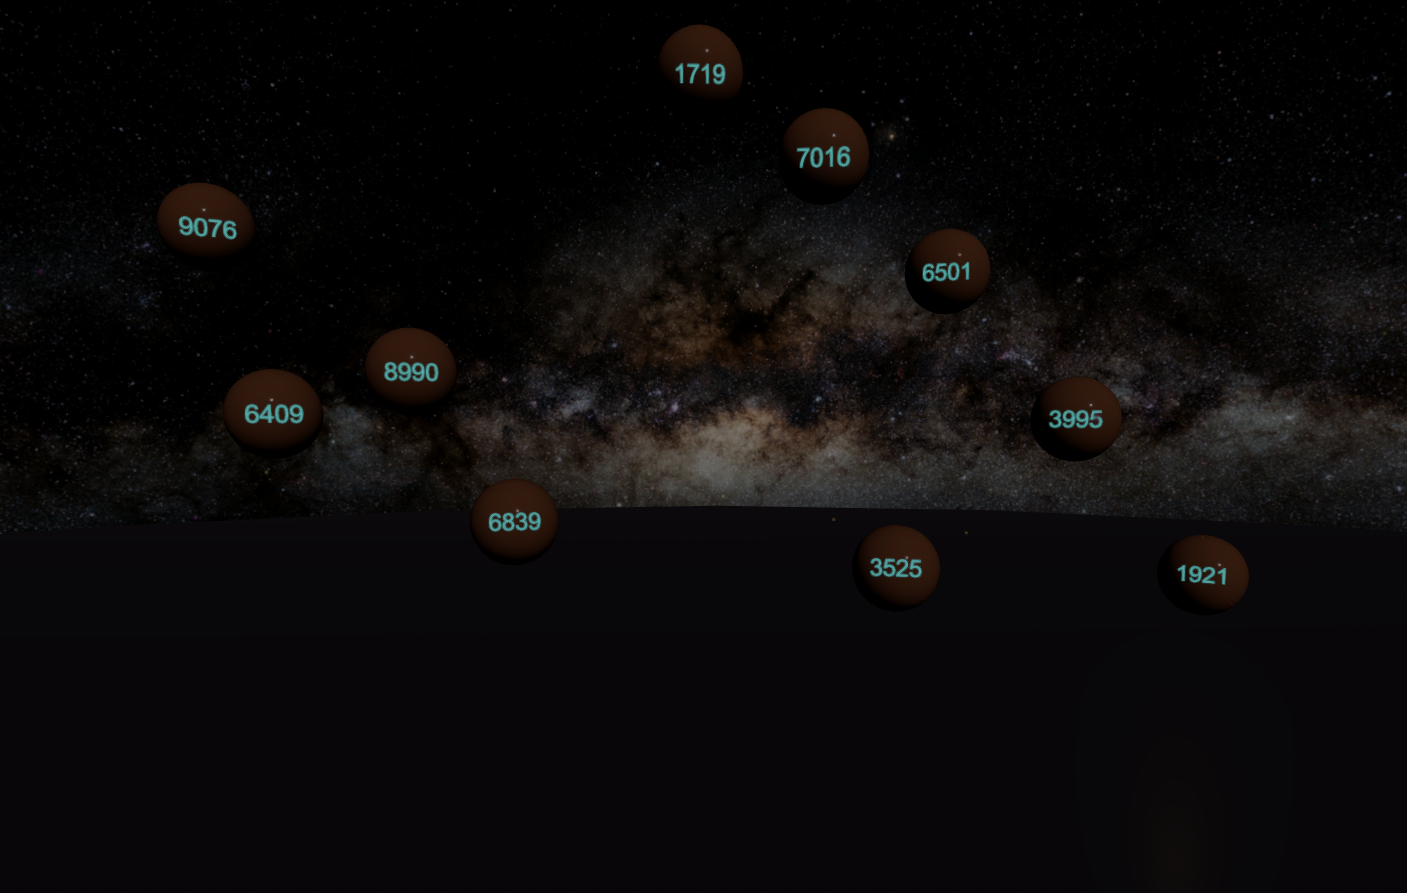
\includegraphics[width=\textwidth]{./images/ordering.png}
		\caption{Erste Aufgabe der Studie.}
		\label{fig:ordering}
	\end{subfigure}%
	\hfill
	\begin{subfigure}{0.48\textwidth}
		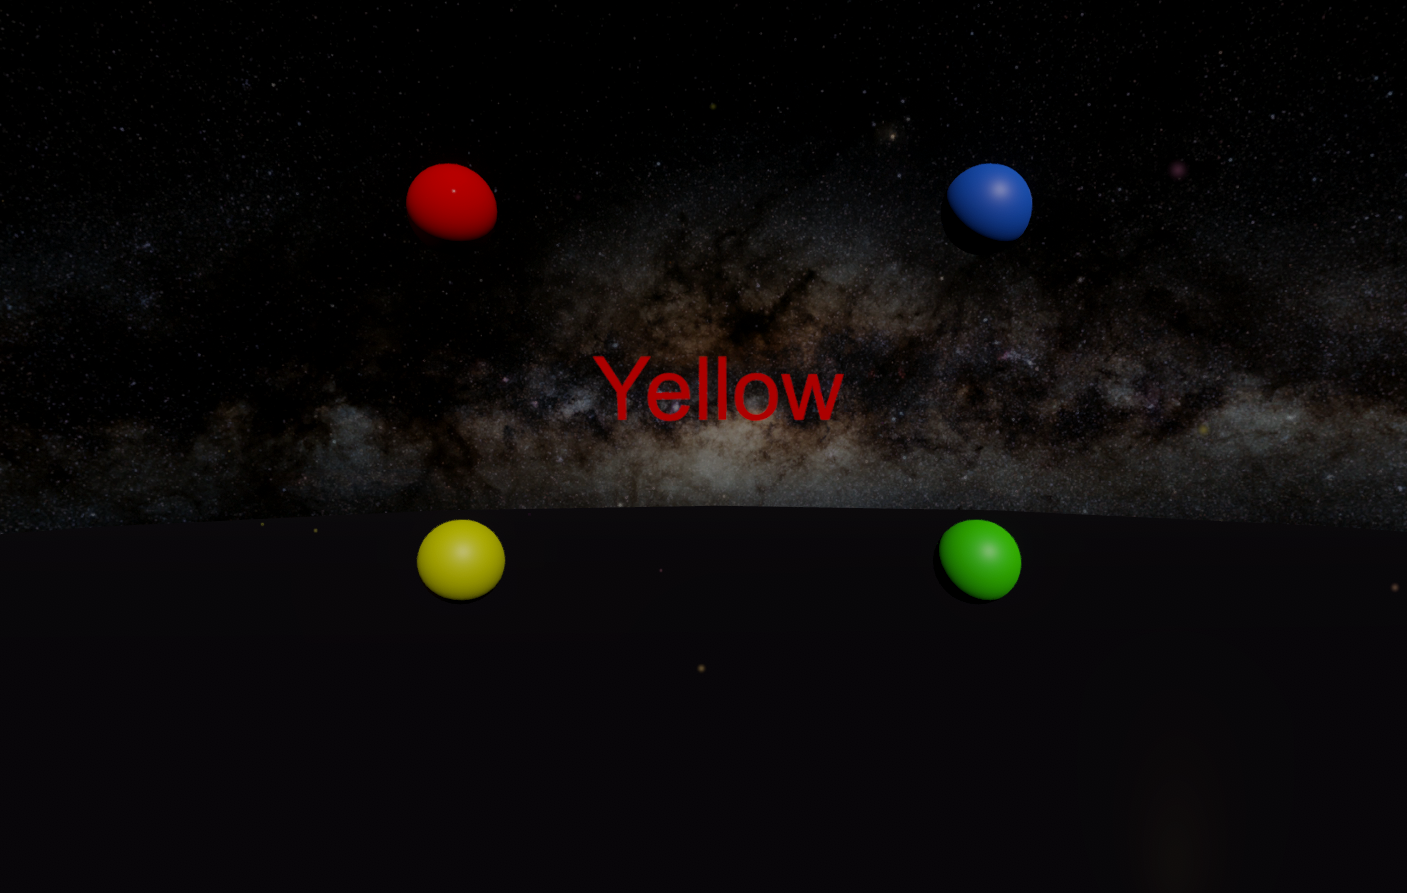
\includegraphics[width=\textwidth]{./images/matching.png}
		\caption{Zweite Aufgabe.}
		\label{fig:matching}
	\end{subfigure}
	\hfill
	\begin{subfigure}{0.48\textwidth}
		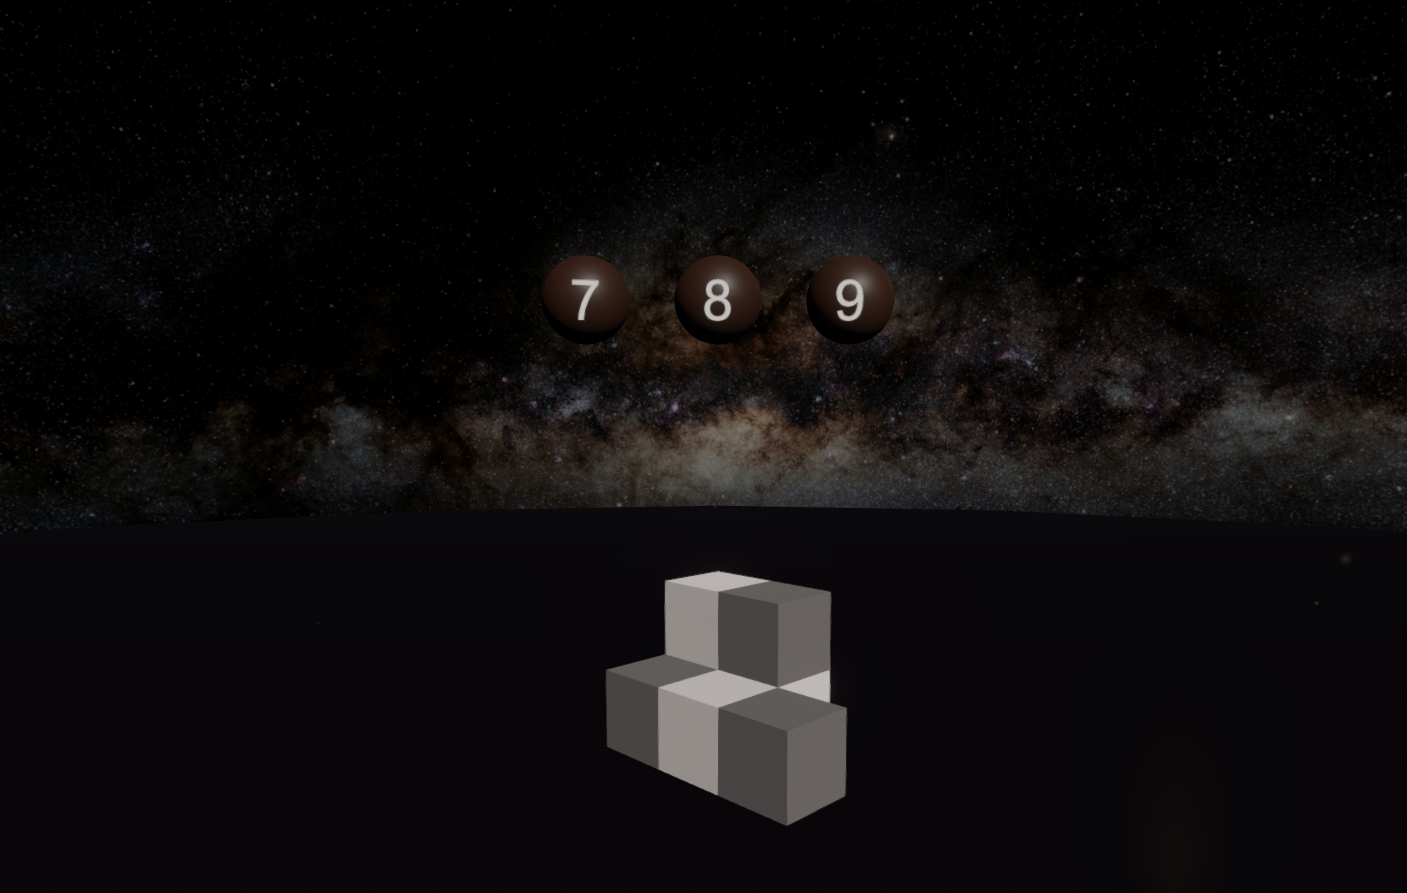
\includegraphics[width=\textwidth]{./images/counting.png}
		\caption{Dritte Aufgabe in der Studie.}
		\label{fig:counting}
	\end{subfigure}
	\caption{Screenshots für die Aufgaben mit denen die Teilnehmer der Studie konfrontiert werden.} % caption for whole figure
\end{figure}

\begin{table*}
	\caption{Numerische Auflistung der Ergebnisse der Frage "`Please select your gender"'.}~\label{tab:sc_results_gender}
	
	\setlength\tabcolsep{3pt}
	\renewcommand{\arraystretch}{1.4}% for the vertical padding
	\begin{tabularx}{\textwidth}{ | x || r | r | }
		\hline
		Geschlecht & Absolutwerte 	& Prozentwerte \\ \hline\hline
		Männlich & 33 & 73.3\% \\ \hline
		Weiblich & 12 & 26.7\% \\ \hline
		Divers & 0 & 0.0\% \\ \hline
	\end{tabularx}
\end{table*}

\begin{table*}
	\caption{Numerische Auflistung der Ergebnisse der Frage "`Please enter your age in years"'.}~\label{tab:sc_results_age}
	
	\setlength\tabcolsep{3pt}
	\renewcommand{\arraystretch}{1.4}% for the vertical padding
	\begin{tabularx}{\textwidth}{ | x | x | x | x | x | x | }
		\hline
		Min & Max & Range & Median & Mean  & Standard Deviation \\ \hline\hline
		19  & 30  & 11    & 23     & 23.04 & 2.53              \\ \hline
	\end{tabularx}
\end{table*}

\begin{table*}
	\caption{Verteilung der Antworten zur Frage "`How much experience do you have with VR?"'.}~\label{tab:sc_results_expVR}
	
	\setlength\tabcolsep{3pt}
	\renewcommand{\arraystretch}{1.4}% for the vertical padding
	\begin{tabularx}{\textwidth}{ | x || r | r | }
		\hline
		Studienfach 						& Absolutwerte 	& Prozentwerte \\ \hline\hline
		[A1] No experience at all 			& 10 			& 22.2\% \\ \hline
		[A2] Almost no experience 			& 15 			& 33.3\% \\ \hline
		[A3] Less than average experience 	& 3 			& 6.7\% \\ \hline
		[A4] Some experience 				& 10 			& 22.2\% \\ \hline
		[A5] More than average experience 	& 2 			& 4.4\% \\ \hline
		[A6] Experienced 					& 2 			& 4.4\% \\ \hline
		[A7] Very highly experienced 		& 3 			& 6.7\% \\ \hline
	\end{tabularx}
\end{table*}

\begin{table*}
	\caption{Numerische Auflistung der Ergebnisse der Frage "`How much experience do you have with VR?"'.}~\label{tab:sc_numbers_expVR}
	
	\setlength\tabcolsep{3pt}
	\renewcommand{\arraystretch}{1.4}% for the vertical padding
	\begin{tabularx}{\textwidth}{ | x | x | x | x | x | x | }
		\hline
		Min & Max & Range & Median & Mean  & Standard Deviation \\ \hline\hline
		1  & 7  & 6    & 2     & 2.93 & 1.78              \\ \hline
	\end{tabularx}
\end{table*}

\begin{table*}
	\caption{Verteilung der Antworten zur Frage "`How much experience do you have with AR?"'.}~\label{tab:sc_results_expAR}
	
	\setlength\tabcolsep{3pt}
	\renewcommand{\arraystretch}{1.4}% for the vertical padding
	\begin{tabularx}{\textwidth}{ | x || r | r | }
		\hline
		Studienfach 						& Absolutwerte 	& Prozentwerte \\ \hline\hline
		[A1] No experience at all 			& 17 			& 37.7\% \\ \hline
		[A2] Almost no experience 			& 10 			& 22.2\% \\ \hline
		[A3] Less than average experience 	& 7 			& 15.5\% \\ \hline
		[A4] Some experience 				& 8 			& 17.7\% \\ \hline
		[A5] More than average experience 	& 2 			& 4.4\% \\ \hline
		[A6] Experienced 					& 1 			& 2.2\% \\ \hline
		[A7] Very highly experienced 		& 0 			& 0.0\% \\ \hline
	\end{tabularx}
\end{table*}

\begin{table*}
	\caption{Numerische Auflistung der Ergebnisse der Frage "`How much experience do you have with AR?"'.}~\label{tab:sc_numbers_expAR}
	
	\setlength\tabcolsep{3pt}
	\renewcommand{\arraystretch}{1.4}% for the vertical padding
	\begin{tabularx}{\textwidth}{ | x | x | x | x | x | x | }
		\hline
		Min & Max & Range & Median & Mean  & Standard Deviation \\ \hline\hline
		1  & 6  & 5    & 2     & 2.36 & 1.38              \\ \hline
	\end{tabularx}
\end{table*}

\begin{table*}
	\caption{Verteilung der Antworten zur Frage "`What subject, if any, did you study or are you currently studying?"'.}~\label{tab:sc_results_study}
	
	\setlength\tabcolsep{3pt}
	\renewcommand{\arraystretch}{1.4}% for the vertical padding
	\begin{tabularx}{\textwidth}{ | x || r | r | }
		\hline
		Studienfach & Absolutwerte & Prozentwerte \\ \hline\hline
		Biologie & 1 & 2.2\% \\ \hline
		Informatik & 8 & 17.8\% \\ \hline
		Informationssystemtechnik & 1 & 2.2\% \\ \hline
		Mathematik & 1 & 2.2\% \\ \hline
		Medieninformatik & 18 & 40.0\% \\ \hline
		Physik & 3 & 6.7\% \\ \hline
		Psychologie & 2 & 4.4\% \\ \hline
		Software Engineering & 8 & 17.8\% \\ \hline
		Wirtschaftsmathematik & 1 & 2.2\% \\ \hline
		Wirtschaftsphysik & 2 & 4.4\% \\ \hline
	\end{tabularx}
\end{table*}

\begin{table*}
	\caption{Verteilung der Einstellungen des Stuhls.}~\label{tab:sc_results_chair}
	
	\setlength\tabcolsep{3pt}
	\renewcommand{\arraystretch}{1.4}% for the vertical padding
	\begin{tabularx}{\textwidth}{ | x || r | r | }
		\hline
		Winkeleinstellungen	in Grad	& Absolutwerte 	& Prozentwerte \\ \hline\hline
		0 							& 7 			& 15.6\% \\ \hline
		30 							& 23			& 51.1\% \\ \hline
		60	 						& 10 			& 22.2\% \\ \hline
		90							& 5 			& 11.1\% \\ \hline
	\end{tabularx}
\end{table*}

\begin{itemize}
	\captionof{anno}{Anmerkungen und Hinweise von Studienteilnehmern}
	\item "`Die Musik war sehr störend, um in einen Ruhezustand zu kommen"'
	\item "`Die VR Umgebung war schön gestaltet, aber die rumschwebenden Partikel waren eher verwirrend, ich dachte ich kann mit diesen interagieren"'
	\item "`Der Stuhl war sehr entspannend und bequem"'
	\item "`Es fiel mir schwer einzuschlafen, da ich zum 1. mal VR gemacht habe und dann neugierig war"'
	\item "`Die Musik war sehr angenehm"'
	\item "`Das lange gedrückt halten zur Interaktion war störend"'
	\item "`haptisches Feedback durch Controller wäre gut gewesen"'
	\item "`Die Brille war sehr unangenehm"'
	\item "`Der Ton fürs Wecken hat mich erschrocken"'
	\item "`Mit meiner Brille war es unangenehm die VR Brille zu tragen"'
	\item "`Ich konnte mich sehr gut entspannen, richtig eingeschlafen bin ich      aber nicht"'
	\item "`Die Interaktion mit dem Controller war sehr intuitiv"'
	\item "`Mir kam die Zeit zum entspannen deutlich länger als 15 Minuten vor "'
	\item "`Egal wie ich die Brille verstellte, richtig scharf konnte ich nie sehen "'
	\item "`Noch fünf bis zehn Minuten länger und ich wäre komplett eingeschlafen "'

\end{itemize}

\begin{table*}
	\caption{Wahrgenommene Schlafdauer.}~\label{tab:sleepduration}
	
	\setlength\tabcolsep{3pt}
	\renewcommand{\arraystretch}{1.4}% for the vertical padding
	\begin{tabularx}{\textwidth}{ | x || r | r | }
		\hline
		wahrgenommene Schlafdauer in min & Absolutwerte & Prozentwerte \\ \hline\hline
		8						   	     & 2			   & 4.4\% \\ \hline
		10   					         & 5			   & 11.1\% \\ \hline
		11						   	     & 1 		   & 2.2\% \\ \hline
		12						   	     & 3			   & 6.7\% \\ \hline
		13							     & 2			   & 4.4\% \\ \hline
		14							     & 1			   & 2.2\% \\ \hline
		10-15	      					 & 3		 & 6.7\% \\ \hline
		15							     & 13		 & 28.9\% \\ \hline
		15-20							 & 1		 & 2.2\% \\ \hline
		17								 & 2		 & 4.4\% \\ \hline
		18								 & 3		 & 6.7\% \\ \hline
		18,5							 & 1		 & 2.2\% \\ \hline
		19								 & 1		 & 2.2\% \\ \hline
		20								 & 6		 & 13.3\% \\ \hline
		30								 & 1		 & 2.2\% \\ \hline
	\end{tabularx}
\end{table*}

\begin{table*}
	\caption{Verteilung der Antworten zur Frage "`Hast du geschlafen?"' .}~\label{tab:sleepstatus}
	
	\setlength\tabcolsep{3pt}
	\renewcommand{\arraystretch}{1.4}% for the vertical padding
	\begin{tabularx}{\textwidth}{ | x || r | r | }
		\hline
		Schlafmodus					& Absolutwerte 	& Prozentwerte \\ \hline\hline
		geschlafen 					& 9 			& 20.0\% \\ \hline
		gedöst/kurz vor eingeschlafen	& 12			& 26.7\% \\ \hline
		meditiert					& 3			& 6.7\% \\ \hline
		nicht geschlafen			& 21 			& 46.7\% \\ \hline
	\end{tabularx}
\end{table*}

\begin{table*}
	\caption{Numerische Auflistung der Ergebnisse der Frage "`RSME"'.}~\label{tab:sc_results_rsme}
	
	\setlength\tabcolsep{3pt}
	\renewcommand{\arraystretch}{1.4}% for the vertical padding
	\begin{tabularx}{\textwidth}{ | x | x | x | x | x | x | }
		\hline
		Min & Max & Range & Median & Mean  & Standard Deviation \\ \hline\hline
		0.13  & 0.66  & 0.53    & 0.27     & 0.28 & 0.11              \\ \hline
	\end{tabularx}
\end{table*}\todoAll{Ich hab vergessen wir die Frage hierbei formuliert haben...?}

\begin{table*}
	\caption{Statistik der Dauer des Alarm-Tons}~\label{tab:times_results_alarm}
	
	\setlength\tabcolsep{3pt}
	\renewcommand{\arraystretch}{1.4}% for the vertical padding
	\begin{tabularx}{\textwidth}{ | x | x | x | x | x | x | }
		\hline
		Min   & Max   & Range & Median  & Mean   & Standard Deviation \\ \hline\hline
		3.91  & 10.84 & 6.93  & 5.87    & 6.60   & 2.18               \\ \hline
	\end{tabularx}
\end{table*}

\begin{table*}
	\caption{Statistik der Fehler von Aufgabe 1: Zahlenfolge.}~\label{tab:sc_results_ordering}
	
	\setlength\tabcolsep{3pt}
	\renewcommand{\arraystretch}{1.4}% for the vertical padding
	\begin{tabularx}{\textwidth}{ | x | x | x | x | x | x | }
		\hline
		Min  & Max   & Range & Median & Mean  & Standard Deviation \\ \hline\hline
		0.00 & 45.00 & 45.00 & 0.00   & 4.24  & 11.31              \\ \hline
	\end{tabularx}
\end{table*}

\begin{table*}
	\caption{Statistik der Fehler von Aufgabe 2: Stroop-Effekt.}~\label{tab:sc_results_matching}
	
	\setlength\tabcolsep{3pt}
	\renewcommand{\arraystretch}{1.4}% for the vertical padding
	\begin{tabularx}{\textwidth}{ | x | x | x | x | x | x | }
		\hline
		Min  & Max   & Range & Median & Mean  & Standard Deviation \\ \hline\hline
		0.00 & 10.00 & 10.00 & 0.00   & 1.29  & 2.87               \\ \hline
	\end{tabularx}
\end{table*}

\begin{table*}
	\caption{Statistik der Fehler von Aufgabe 3: Boxen zählen.}~\label{tab:sc_results_counting}
	
	\setlength\tabcolsep{3pt}
	\renewcommand{\arraystretch}{1.4}% for the vertical padding
	\begin{tabularx}{\textwidth}{ | x | x | x | x | x | x | }
		\hline
		Min  & Max   & Range & Median & Mean  & Standard Deviation \\ \hline\hline
		0.00 & 2.00  & 2.00  & 0.00   & 0.31  & 0.60               \\ \hline
	\end{tabularx}
\end{table*}

\begin{table*}
	\caption{Statistik der Dauer bis zur Erledigung von Aufgabe 1: Zahlenfolge in Sekunden.}~\label{tab:times_results_ordering}
	
	\setlength\tabcolsep{3pt}
	\renewcommand{\arraystretch}{1.4}% for the vertical padding
	\begin{tabularx}{\textwidth}{ | x | x | x | x | x | x | }
		\hline
		Min   & Max   & Range & Median  & Mean   & Standard Deviation \\ \hline\hline
		16.59 & 43.49 & 26.90 & 25.55   & 26.80  & 6.25               \\ \hline
	\end{tabularx}
\end{table*}

\begin{table*}
	\caption{Statistik der Dauer bis zur Erledigung von Aufgabe 2: Stroop-Effekt in Sekunden.}~\label{tab:times_results_ordering}
	
	\setlength\tabcolsep{3pt}
	\renewcommand{\arraystretch}{1.4}% for the vertical padding
	\begin{tabularx}{\textwidth}{ | x | x | x | x | x | x | }
		\hline
		Min   & Max   & Range & Median  & Mean   & Standard Deviation \\ \hline\hline
		13.87 & 83.31 & 69.44 & 20.70   & 24.23  & 11.13              \\ \hline
	\end{tabularx}
\end{table*}

\begin{table*}
	\caption{Statistik der Dauer bis zur Erledigung von Aufgabe 3: Boxen zählen in Sekunden.}~\label{tab:times_results_ordering}
	
	\setlength\tabcolsep{3pt}
	\renewcommand{\arraystretch}{1.4}% for the vertical padding
	\begin{tabularx}{\textwidth}{ | x | x | x | x | x | x | }
		\hline
		Min   & Max   & Range & Median  & Mean   & Standard Deviation \\ \hline\hline
		15.34 & 54.15 & 38.82 & 31.72   & 32.75  & 9.63               \\ \hline
	\end{tabularx}
\end{table*}

\begin{table*}
	\caption{Detaillierte Statistik der Zeiten zu Aufgabe 1: Zahlenfolge in Millisekunden.}~\label{tab:times_ordering}
	
	\setlength\tabcolsep{3pt}
	\renewcommand{\arraystretch}{1.4}% for the vertical padding
	\begin{tabularx}{\textwidth}{ | l | x | x | x | x | x | x | }
		\hline
		Objekt 	& Min   & Max   & Range & Median  & Mean    & Standard Deviation \\ \hline\hline
		1 		& 1626  & 23307 & 21681 & 5329    & 6418.36 & 3768.54            \\ \hline
		2 		& 590   & 8618  & 8028  & 2466    & 2697.87 & 1551.57            \\ \hline
		3 		& 1266  & 9550  & 8284  & 4054    & 4045.69 & 1753.47            \\ \hline
		4 		& 745   & 16870 & 16125 & 1710    & 2358.60 & 2491.20            \\ \hline
		5 		& 723   & 9141  & 8418  & 3565    & 4226.16 & 2076.30            \\ \hline
		6 		& 668   & 5399  & 4731  & 1445    & 1553.13 & 751.37             \\ \hline
		7 		& 456   & 3853  & 3397  & 1466    & 1773.02 & 842.58             \\ \hline
		8 		& 723   & 3409  & 2686  & 1388    & 1605.80 & 649.10             \\ \hline
		9 		& 422   & 2096  & 1674  & 1077    & 1164.02 & 425.17             \\ \hline
		10 		& 545   & 1532  & 987   & 944     & 957.42  & 245.02             \\ \hline
	\end{tabularx}
\end{table*}
